\documentclass[onecolumn]{emulateapj}

% Load commands
\input{my_defs.defs}

% Load packages
\usepackage{color, colortbl}
\definecolor{Gray}{gray}{0.85}
\usepackage{enumerate}
\usepackage{graphicx}
\usepackage{float}
\usepackage{multirow}

% bibtex entries
\usepackage{natbib}
\bibliographystyle{apj}

\begin{document}

\slugcomment{Last edited\today}

%-----------------------------------------------------------------------------%
\title{Literature Review Notes Document}
%-----------------------------------------------------------------------------%

%-----------------------------------------------------------------------------%
% Author list 
%-----------------------------------------------------------------------------%

\author{
  Elijah Bernstein-Cooper \altaffilmark{1}, 
}

\altaffiltext{1}{UW Madison}

\keywords{example: another --- one more}

%=============================================================================%
%-----------------------------------------------------------------------------%
\begin{abstract}
%-----------------------------------------------------------------------------%
%=============================================================================%

This is for lit reviews

\end{abstract}

%=============================================================================%
%-----------------------------------------------------------------------------%
\section{Introduction}
  \label{sec: introduction}
%-----------------------------------------------------------------------------%
%=============================================================================%

Cite things from mybib.bib \citet{mcconnachie2009}.

Use defs like \hi\ from my_defs.defs.

%-------------------------------------------------------------------------------
\begin{table}[!ht]
  \centering TABLE \ref{table: }\\ 
  
  \textsc{Example table}\\
  
  \label{table: }
  \vspace{.5cm}
  \begin{tabular}{lc}

      Sample header & header  \\ 

\hline \hline
%-------------------------------------------------------------------------------

sample column & sample column \\ % \tablenotemark{a}\\ \rowcolor{Gray}

  \end{tabular}

  %\tablenotetext{a}{Properties from \citet{mcconnachie2012}}

\end{table} 
%-------------------------------------------------------------------------------

%------------------------------------------------------------------------------
\begin{figure}[!ht]
  \begin{center}
  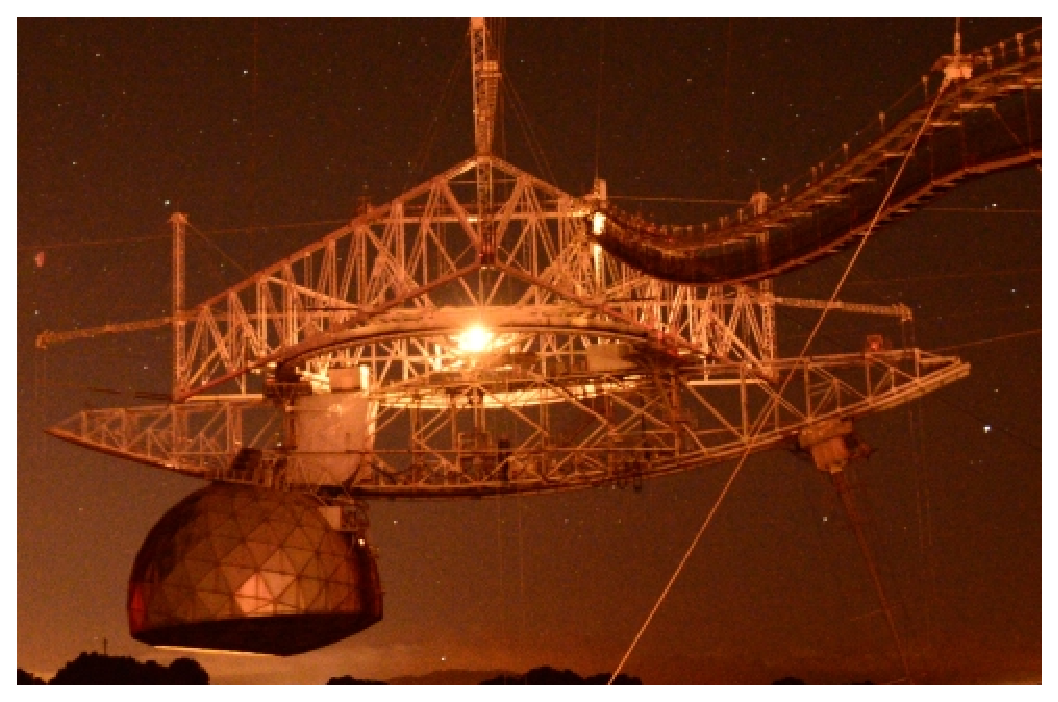
\includegraphics[scale=0.2]{figures/test_figure.eps}
  %\plotone{figures/test_figure.png}

  \caption{Example plot}

  \label{fig: }
  \end{center}
\end{figure}
%-------------------------------------------------------------------------------

\bibliography{my_bib.bib}

%-----------------------------------------------------------------------------%

\end{document}
